\documentclass[xcolor=dvipsnames]{beamer}

\makeatletter

%HAY QUE ELEGIR EL QUE CORRESPONDA

%\usepackage{mathpazo}%Letra palatino con fuentes para matemáticas
\usepackage[T1]{fontenc}
\usepackage[utf8]{inputenc}
\usepackage{graphicx}
\usepackage{url}
\usepackage{amsmath}
\usepackage{booktabs}
\usepackage{textcomp}%%needed for the euro symbol

\date{}

\usepackage[emulate=units]{siunitx}
\sisetup{per=fraction, fraction=nice, decimalsymbol=comma}
\newunit{\wattpeak}{Wp}
\newunit{\watthour}{Wh}
\newunit{\amperehour}{Ah}

\setbeamercovered{transparent}
\setbeamertemplate{navigation symbols}{}
\usefonttheme{structuresmallcapsserif} 
\usefonttheme{serif} 
\usefonttheme{structurebold}

%\usepackage{epstopdf}


\usepackage[spanish]{babel}
\addto\shorthandsspanish{\spanishdeactivate{~<>}}

\hypersetup{pdfauthor={Oscar Perpi\~n\'an},%
    pdftitle={Energ\'ia Solar Fotovoltaica},%
    filecolor=blue,%
    urlcolor=blue}



%\usepackage{handoutWithNotes} %para hacer papel con notas 
%\pgfpagesuselayout{4 on 1 with notes}[a4paper,border shrink=5mm]



%\usepackage{pgfpages}
%\pgfpagesuselayout{2 on 1}[a4paper,border shrink=5mm]


%\usepackage{mathpazo}%Letra palatino con fuentes para matemáticas
\usepackage[T1]{fontenc}
\usepackage[utf8]{inputenc}
\usepackage{graphicx}
\usepackage{url}
\usepackage{amsmath}
\usepackage{booktabs}

\usepackage[spanish]{babel}
\addto\shorthandsspanish{\spanishdeactivate{~<>}}


\usepackage{hyperref}
% \hypersetup{pdfauthor={Oscar Perpi\~n\'an},%
%     pdftitle={Energ\'ia Solar Fotovoltaica},%
%     filecolor=blue,%
%     urlcolor=blue}

\hypersetup{
    bookmarks=true,         % show bookmarks bar?
%    unicode=true,          % non-Latin characters in Acrobat’s bookmarks
    bookmarksnumbered=false,
    bookmarksopen=false,
    breaklinks=true,
    backref=true,
    pdftoolbar=true,        % show Acrobat’s toolbar?
    pdfmenubar=true,        % show Acrobat’s menu?
    pdffitwindow=false,     % window fit to page when opened
    pdfstartview={FitH},    % fits the width of the page to the window
    pdftitle={Energía Solar Fotovoltaica},    % title
    pdfauthor={Oscar Perpiñán Lamigueiro},     % author
    pdfsubject={Electrotecnia},   % subject of the document
    pdfcreator={AucTeX/Emacs},   % creator of the document
    pdfproducer={LaTeX}, % producer of the document
    pdfnewwindow=true,      % links in new window
    pdfborder={0 0 0},
    colorlinks=true,       % false: boxed links; true: colored links
    linkcolor=,          % color of internal links
    citecolor=BrickRed,        % color of links to bibliography
    filecolor=black,      % color of file links
    urlcolor=Blue           % color of external links 
}

\usepackage[emulate=units]{siunitx}
\sisetup{per=fraction, fraction=nice, decimalsymbol=comma}
\newunit{\wattpeak}{Wp}
\newunit{\watthour}{Wh}
\newunit{\amperehour}{Ah}

\setbeamercovered{transparent}
\setbeamertemplate{navigation symbols}{}
\usefonttheme{serif} 
\usefonttheme{structuresmallcapsserif} 

\useinnertheme[shadow=true]{rounded}
\useoutertheme{shadow}
%\usecolortheme[named=BrickRed]{structure} %sirve para cambiar el color genérico
\usecolortheme{orchid}
\usecolortheme{whale}
\documentclass[xcolor={usenames,svgnames,dvipsnames}]{beamer}
\usepackage[utf8]{inputenc}
\usepackage[T1]{fontenc}
\usepackage{graphicx}
\usepackage{grffile}
\usepackage{longtable}
\usepackage{wrapfig}
\usepackage{rotating}
\usepackage[normalem]{ulem}
\usepackage{amsmath}
\usepackage{textcomp}
\usepackage{amssymb}
\usepackage{capt-of}
\usepackage{hyperref}
\usepackage{color}
\usepackage{listings}
\usepackage{mathpazo}
\usepackage{gensymb}
\usepackage{amsmath}
\usepackage{chemarr}%flechas para reacciones químicas (SFER.tex)
\bibliographystyle{plain}
\AtBeginSubsection[]{\begin{frame}[plain]\tableofcontents[currentsubsection,sectionstyle=show/shaded,subsectionstyle=show/shaded/hide]\end{frame}}
\AtBeginSection[]{\begin{frame}[plain]\tableofcontents[currentsection,hideallsubsections]\end{frame}}
\usepackage[emulate=units]{siunitx}
\sisetup{fraction=nice, decimalsymbol=comma, retain-unity-mantissa = false}
\newunit{\wattpeak}{Wp}
\newunit{\watthour}{Wh}
\newunit{\amperehour}{Ah}
\usepackage{steinmetz}
\hypersetup{colorlinks=true, linkcolor=OliveGreen, urlcolor=Blue}
\renewcommand{\thefootnote}{\fnsymbol{footnote}}
\beamertemplatenavigationsymbolsempty
\setbeamertemplate{footline}[frame number]

\setbeamercolor{alerted text}{fg=Green!50!black} \setbeamerfont{alerted text}{series=\bfseries}
\usefonttheme{serif}
\setbeamercovered{transparent}
\setbeamertemplate{navigation symbols}{}
\usefonttheme{serif} 

\setbeamercolor{palette primary}{bg=OliveGreen,fg=white}
\setbeamercolor{palette secondary}{bg=OliveGreen,fg=white}
\setbeamercolor{palette tertiary}{bg=OliveGreen,fg=white}
\setbeamercolor{palette quaternary}{bg=OliveGreen,fg=white}
\setbeamercolor{structure}{fg=OliveGreen} % itemize, enumerate, etc
\setbeamercolor{section in toc}{fg=OliveGreen} % TOC sections

\usetheme[hideothersubsections]{Goettingen}

\usepackage{tikz}

\titlegraphic{
\includegraphics[width=2.5cm]{../figs/logoEOI.jpg}}
\addtobeamertemplate{frametitle}{}{%
\begin{tikzpicture}[remember picture,overlay]
\node[anchor=south east,yshift=2pt] at (current page.south east) {
\includegraphics[width=1.5cm]{../figs/logoEOI.jpg}};
\end{tikzpicture}}


\makeatother


\begin{document}


\title{\textsc{Energía Solar Fotovoltaica:}\\
  \textsc{Geometría Solar}}


\author{\textsc{Oscar Perpiñán Lamigueiro}}

\date{}


\begin{frame}[plain]
  \titlepage
\end{frame}

\AtBeginSection[]{
  \begin{frame}[plain]
    \frametitle{Índice}
    % \setcounter{tocdepth}{1}
    \tableofcontents[currentsection]
  \end{frame}

}

\selectlanguage{spanish}%


\section{Movimiento Sol y Tierra}



\begin{frame}
  \frametitle{Movimiento Sol-Tierra}
  \begin{itemize}
  \item La Tierra se mueve alrededor del Sol siguiendo una elipse de
    baja excentricidad.

    \begin{itemize}
    \item Periodo aproximado: 1 año.
    \item Este movimiento está contenido en el llamado \emph{plano de
        la eclíptica}
    \end{itemize}
  \item La Tierra gira sobre si misma alrededor de su eje polar.

    \begin{itemize}
    \item Entre el eje polar y el plano de la eclíptica hay un ángulo
      constante de $23,45\degree$.
    \item Entre el plano ecuatorial y la linea que une Tierra-Sol hay
      un ángulo variable: \emph{declinación.}
    \end{itemize}
  \end{itemize}

\end{frame}


\begin{frame}
  \frametitle{Movimiento Sol-Tierra}

  \begin{center}
    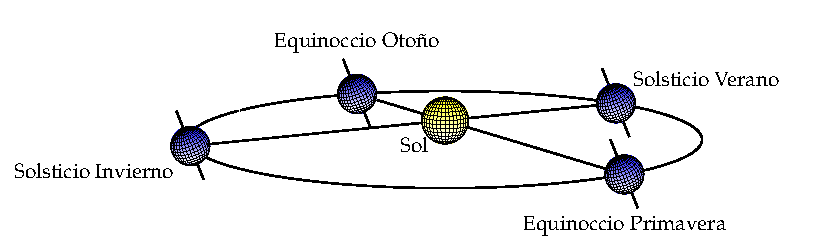
\includegraphics[scale=0.8]{../Figuras/PlanoEcliptica}
    \par\end{center}


\end{frame}

\begin{frame}
  \frametitle{Distancia Sol-Tierra}

  Distancia Sol-Tierra

\[
r=r_{0}\{1+0.017\sin[\frac{2\pi\cdot(d_{n}-93)}{365}]\}\]


Distancia promedio

\[
r_{0}=\SI{1.496e8}{\kilo\metre}=\SI{1}{UA}\]


Excentricidad

\[
\epsilon_{0}=(\frac{r_{0}}{r})^2=1+0,033\cdot\cos(\frac{2\pi
  d_{n}}{365})\]



\end{frame}

\begin{frame}[plain]
  \frametitle{Declinación}

\[
\delta=23,45\degree\cdot\sin\left(\frac{2\pi\cdot\left(d_{n}+284\right)}{365}\right)\]


\begin{center}
  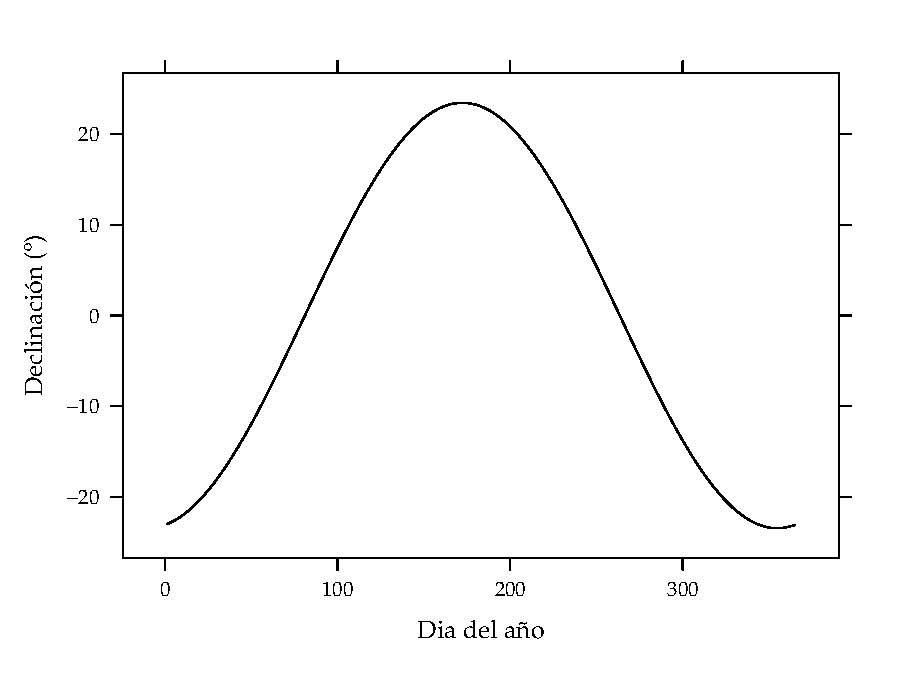
\includegraphics[scale=0.6]{../Figuras/Declinacion}
  \par\end{center}


\end{frame}

\begin{frame}
  \frametitle{Otras ecuaciones}
  \begin{align*}
    \label{eq:spencer}
    X &= 2 \pi \cdot (d_n-1)/365\\
    \begin{split}
      \delta &= 0.006918 - 0.399912 \cdot \cos(X) + 0.070257 \cdot \sin(X)\\
      &-  0.006758 \cdot \cos(2 X) + 0.000907 \cdot \sin(2 X)\\
      &- 0.002697 \cdot \cos(3 X) + 0.001480 \cdot \sin(3 X)
    \end{split}\\
    \begin{split}
      \epsilon_{0} &= 1.000110 + 0.034221 \cdot \cos(X) + 0.001280
      \cdot
      \sin(X)\\
      &+ 0.000719 \cdot \cos(2 X) + 0.000077 \cdot \sin(2 X)
    \end{split}
  \end{align*}
\end{frame}

\begin{frame}
  \frametitle{Otras ecuaciones}
  \begin{center}
    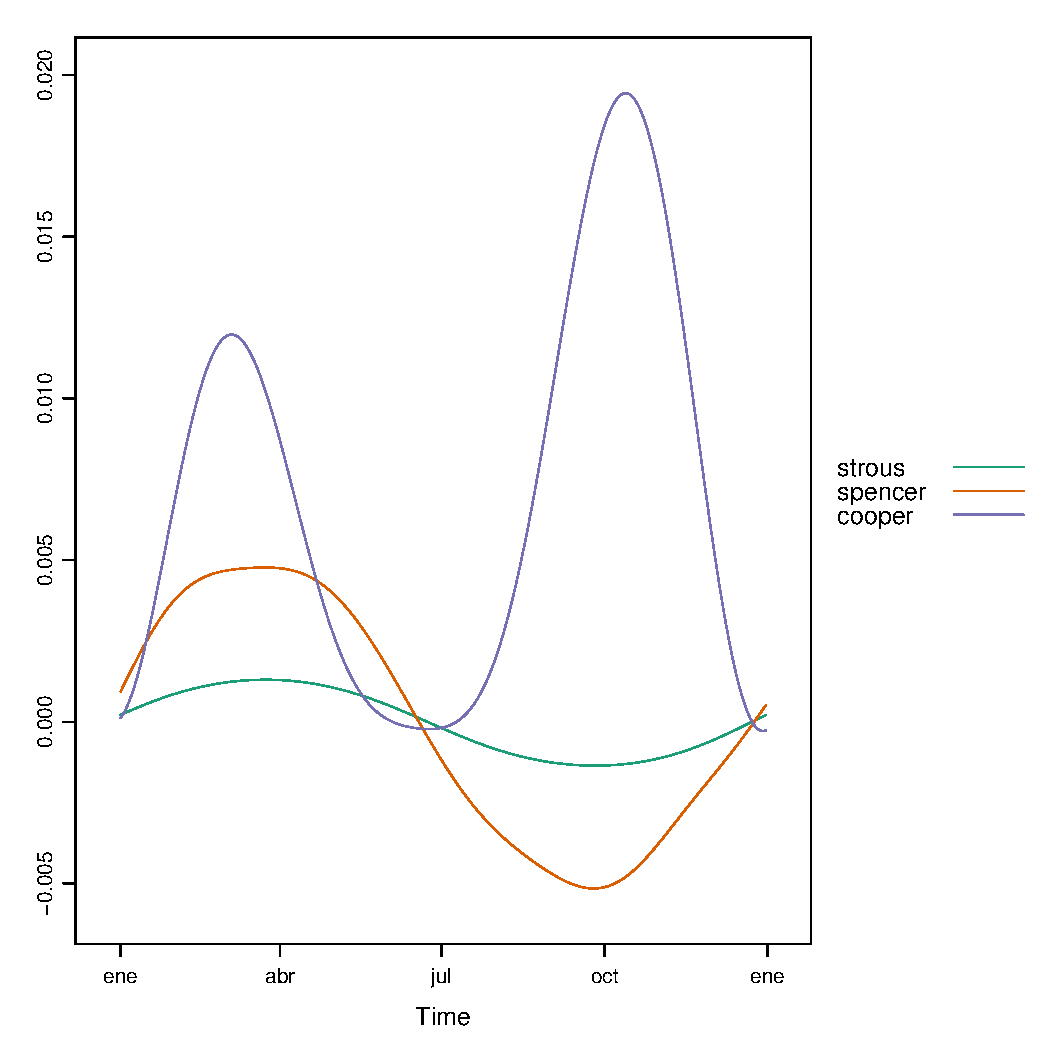
\includegraphics[height=0.85\textheight,keepaspectratio]{../Figuras/DeclinacionDiferencias}
  \end{center}
\end{frame}

\begin{frame}
  \frametitle{Declinación}
  \begin{itemize}
  \item \textbf{Equinoccio de primavera}:

    \begin{itemize}
    \item 21-22 Marzo (Dia del Año 80-81)
    \end{itemize}
  \item \textbf{Equinoccio de otoño:}

    \begin{itemize}
    \item 22-23 Septiembre (Dia del Año 265-266)
    \end{itemize}
  \item \textbf{Solsticio de Verano}:

    \begin{itemize}
    \item 21-22 Junio (Dia del Año 172-173)
    \end{itemize}
  \item \textbf{Solsticio de Invierno:}

    \begin{itemize}
    \item 21-22 Diciembre (Dia del Año 355-356)
    \end{itemize}
  \end{itemize}

\end{frame}

\begin{frame}
  \frametitle{Declinación}
  \begin{itemize}
  \item Las estaciones se deben al ángulo entre plano ecuatorial y
    plano de la eclíptica
  \item \textbf{Solsticio de verano}

    \begin{itemize}
    \item Declinación máxima.
    \item Días más largos en hemisferio Norte.
    \item El Sol amanece por el Noreste y anochece por el Noroeste en
      el hemisferio Norte.
    \end{itemize}
  \item \textbf{Solsticio de invierno}

    \begin{itemize}
    \item Declinación mínima.
    \item Días más cortos en hemisferio Norte.
    \item El Sol amanece por el Sureste y anochece por el Suroeste en
      el hemisferio Norte.
    \end{itemize}
  \item \textbf{Equinoccios}

    \begin{itemize}
    \item Declinación nula
    \item La duración de noche y día coincide.
    \item El Sol amanece por el Este y anochece por el Oeste.
    \end{itemize}
  \end{itemize}



\end{frame}

\begin{frame}[plain]
  \frametitle{Ejes terrestres}

  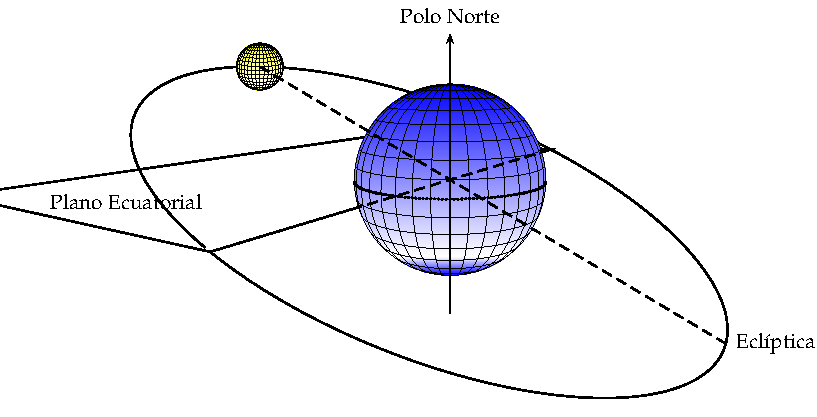
\includegraphics[scale=0.8]{../Figuras/SoldesdeTierra}

\[
\vec{\mu}_{s}=\left[\cos\left(\delta\right)\cos\left(\omega\right)\right]\cdot\vec{\mu}_{ec}+\left[\cos\left(\delta\right)\sin\left(\omega\right)\right]\cdot\vec{\mu}_{\bot}+\sin\left(\delta\right)\cdot\vec{\mu}_{p}\]



\end{frame}

\begin{frame}[plain]
  \frametitle{Ejes terrestres}

\[
\vec{\mu}_{s}=\left[\cos\left(\delta\right)\cos\left(\omega\right)\right]\cdot\vec{\mu}_{ec}+\left[\cos\left(\delta\right)\sin\left(\omega\right)\right]\cdot\vec{\mu}_{\bot}+\sin\left(\delta\right)\cdot\vec{\mu}_{p}\]


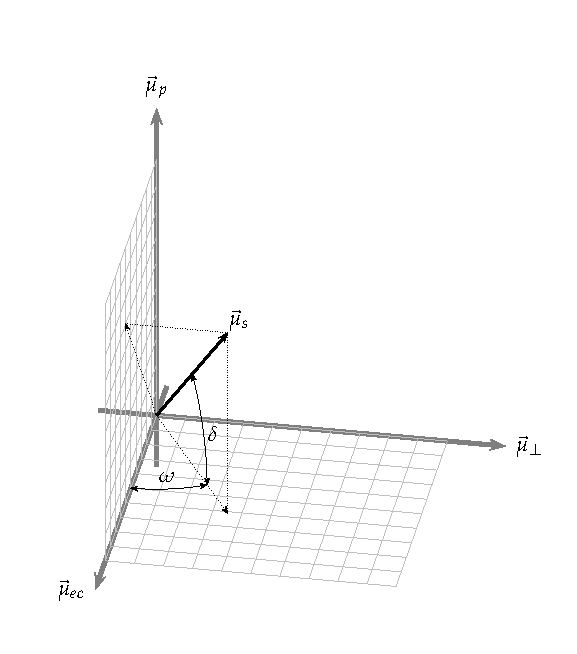
\includegraphics[scale=0.7]{../Figuras/SistemaCoordenadasTerrestre}


\end{frame}

\begin{frame}[plain]
  \frametitle{Ejes locales}

  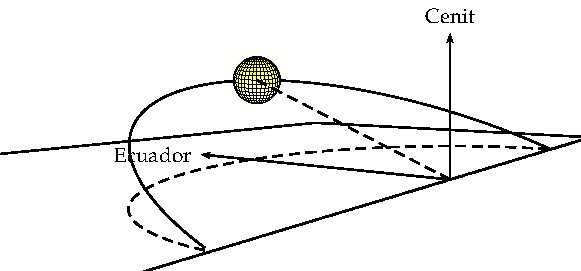
\includegraphics{../Figuras/SoldesdeTierra2}

\[
\vec{\mu}_{s}=\left[\cos\left(\psi_{s}\right)\sin\left(\theta_{z}\right)\right]\cdot\vec{\mu}_{h}+\left[\sin\left(\psi_{s}\right)\sin\left(\theta_{z}\right)\right]\cdot\vec{\mu}_{\bot}+\cos\left(\theta_{z}\right)\cdot\vec{\mu}_{c}\]



\end{frame}

\begin{frame}[plain]
  \frametitle{Ejes locales}

  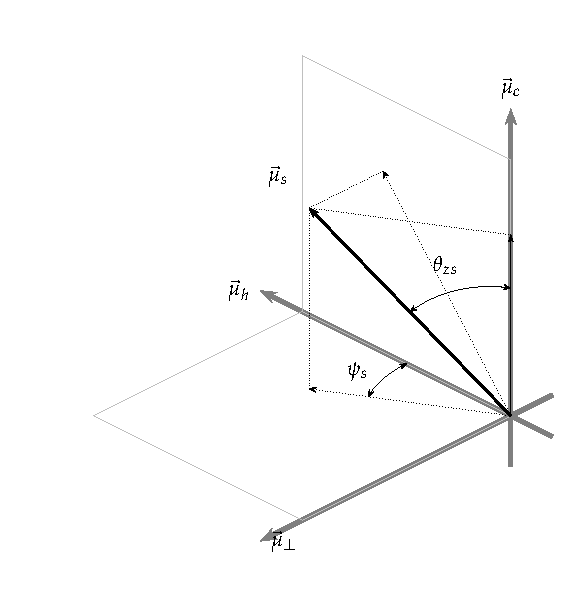
\includegraphics[scale=0.7]{../Figuras/SistemaCoordenadasLocal}

\[
\vec{\mu}_{s}=\left[\cos\left(\psi_{s}\right)\sin\left(\theta_{z}\right)\right]\cdot\vec{\mu}_{h}+\left[\sin\left(\psi_{s}\right)\sin\left(\theta_{z}\right)\right]\cdot\vec{\mu}_{\bot}+\cos\left(\theta_{z}\right)\cdot\vec{\mu}_{c}\]


\end{frame}

\begin{frame}
  \frametitle{Relación entre sistemas de coordenadas}

  \begin{center}
    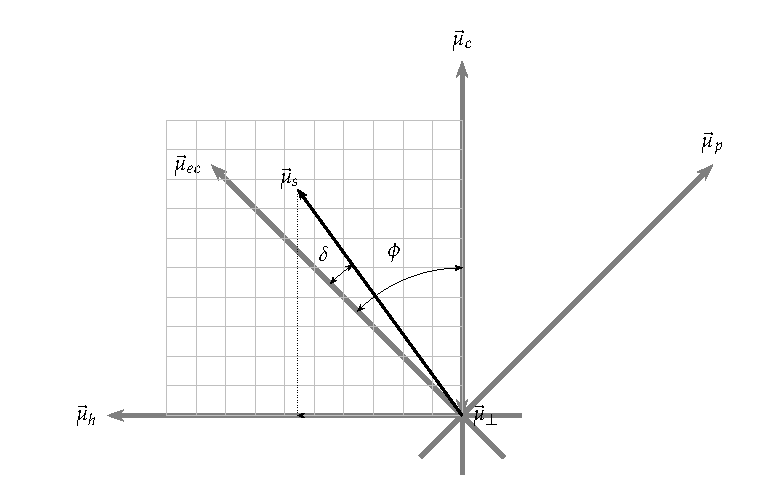
\includegraphics[scale=0.8]{../Figuras/RelacionSistemasCoordenadas}
    \par\end{center}




\end{frame}

\begin{frame}
  \frametitle{Ejes locales y terrestres}

\begin{align}
  \vec{\mu}_{s} & =\mathrm{signo}(\phi)\cdot\left[\cos\left(\delta\right)\cos\left(\omega\right)\sin\left(\phi\right)-\cos\left(\phi\right)\sin\left(\delta\right)\right]\cdot\vec{\mu}_{h}-\nonumber \\
  & -\left[\cos\left(\delta\right)\sin\left(\omega\right)\right]\cdot\vec{\mu}_{\bot}+\\
  &
  +\left[\cos\left(\delta\right)\cos\left(\omega\right)\cos\left(\phi\right)+\sin\left(\delta\right)\sin\left(\phi\right)\right]\cdot\vec{\mu}_{c}\nonumber \end{align}
\begin{block}{}
  \textbf{Latitud ($\phi$) con signo}: Positivo para Hemisferio Norte,
  Negativo para Hemisferio Sur.
\end{block}

\end{frame}

\begin{frame}
  \frametitle{Ángulos Solares}

\[
\cos\left(\theta_{z}\right)=\vec{\mu}_{c}\cdot\vec{\mu}_{s}=\cos\left(\delta\right)\cos\left(\omega\right)\cos\left(\phi\right)+\sin\left(\delta\right)\sin\left(\phi\right)\]

\begin{align*}
  \vec{\mu_{s}}\cdot\vec{\mu}_{\bot} & =-\sin\left(\psi_{s}\right)\sin\left(\theta_{zs}\right)\\
  \vec{\mu_{s}}\cdot\vec{\mu}_{h} & =\mathrm{signo}(\phi)\cdot\cos\left(\psi_{s}\right)\sin\left(\theta_{zs}\right)\\
  \cos\left(\psi_{s}\right) & =\mathrm{signo}(\phi)\cdot\frac{\cos\left(\delta\right)\cos\left(\omega\right)\sin\left(\phi\right)-\cos\left(\phi\right)\sin\left(\delta\right)}{\sin\left(\theta_{zs}\right)}\\
  \sin(\psi_{s}) &
  =\frac{\cos(\delta)\sin(\omega)}{\sin(\theta_{zs})}=\frac{\cos(\delta)\sin(\omega)}{\cos(\gamma_{s})}\end{align*}



\end{frame}

\begin{frame}[plain]
  \frametitle{Altura Solar (hemisferio NORTE)}

  \begin{center}
    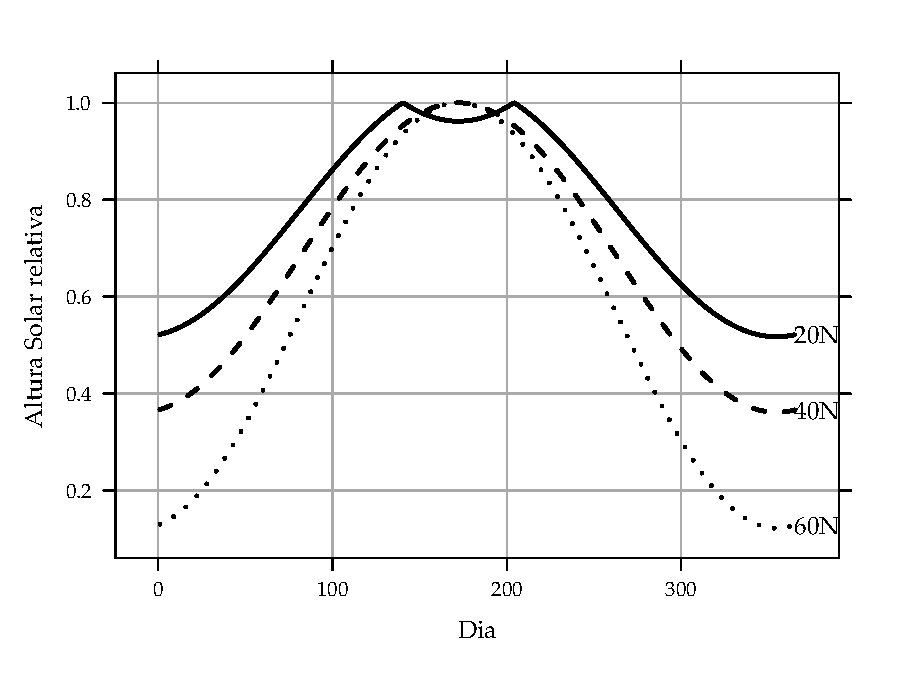
\includegraphics[scale=0.6]{../Figuras/AlturaSolarMediodiaNORTE}
    \par\end{center}


\end{frame}

\begin{frame}[plain]
  \frametitle{Altura Solar (hemisferio SUR)}

  \begin{center}
    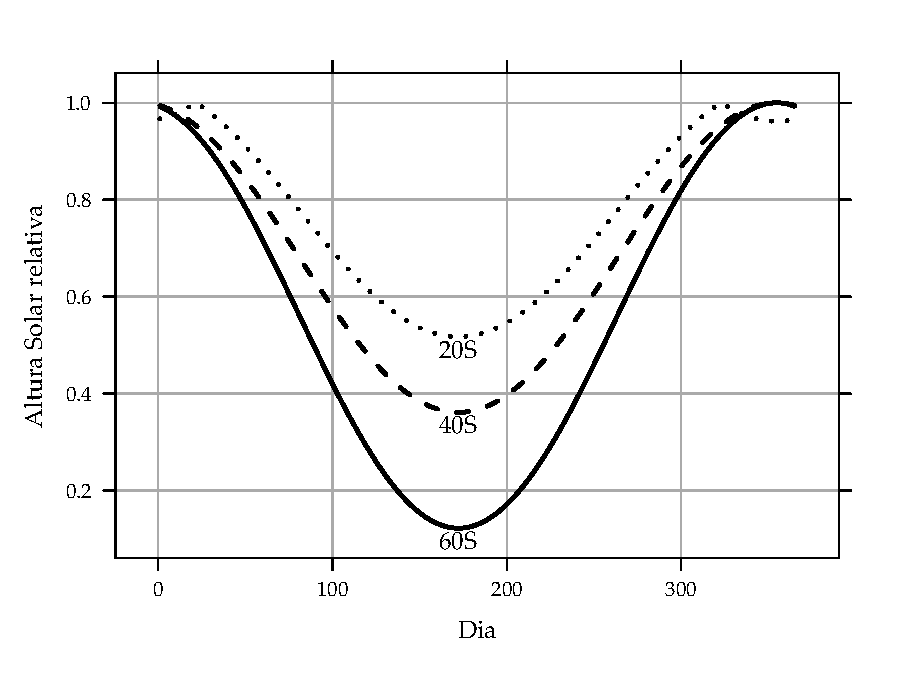
\includegraphics[scale=0.6]{../Figuras/AlturaSolarMediodiaSUR}
    \par\end{center}


\end{frame}

\begin{frame}[plain]
  \frametitle{Trayectoria Solar ($60\degree N$)}

  \begin{center}
    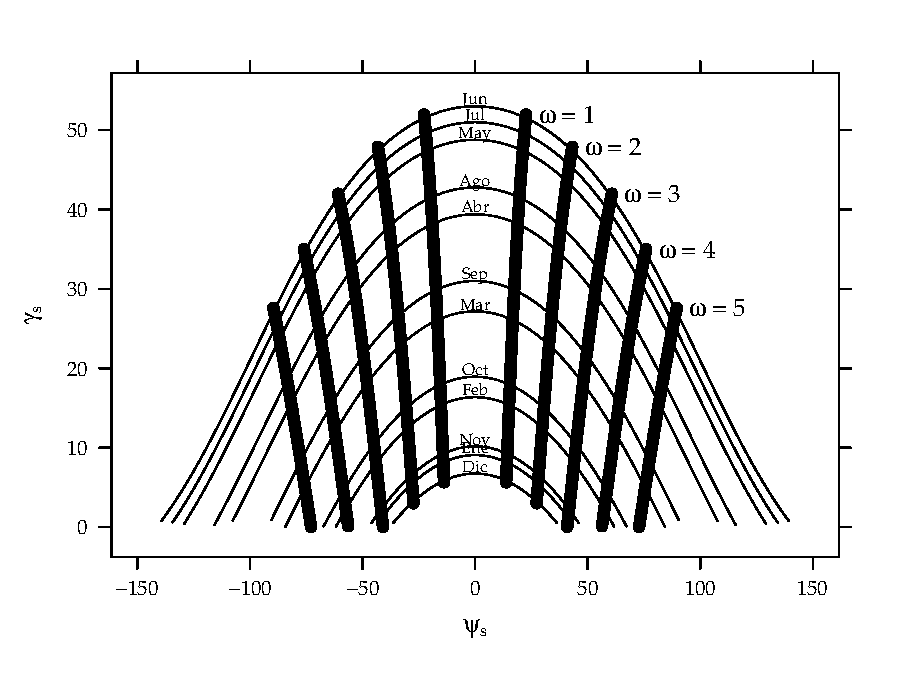
\includegraphics[scale=0.6]{../Figuras/TrayectoriaSolar60N}
    \par\end{center}


\end{frame}

\begin{frame}[plain]
  \frametitle{Trayectoria Solar ($40\degree S$)}

  \begin{center}
    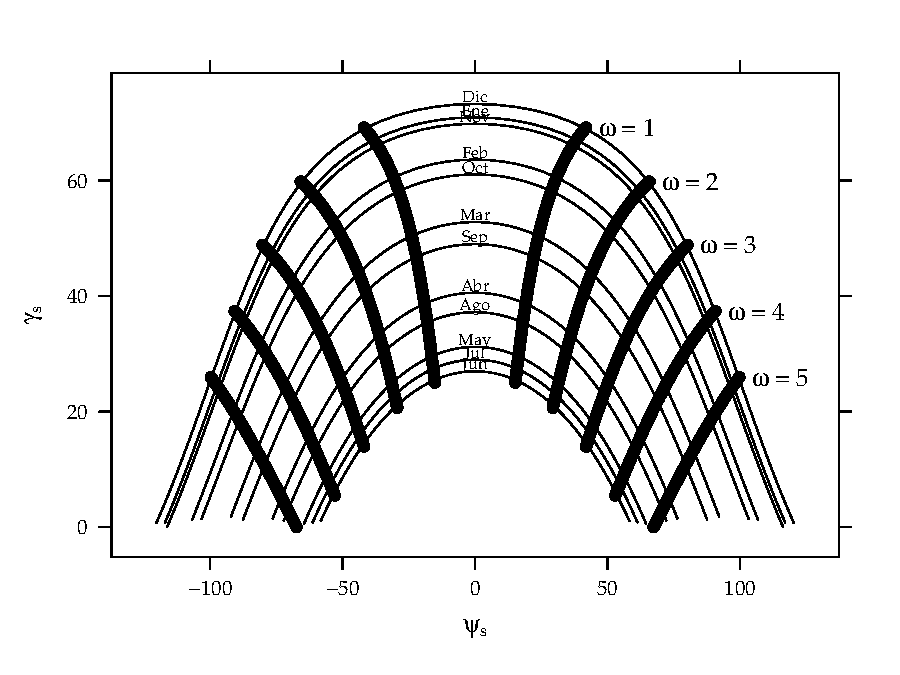
\includegraphics[scale=0.6]{../Figuras/TrayectoriaSolar40S}
    \par\end{center}


\end{frame}

\begin{frame}
  \frametitle{Mediodía, amanecer y anocher}
  \begin{itemize}
  \item Mediodía: \[
    \psi_{s}=0\Rightarrow\sin(\psi_{s})\Rightarrow\omega=0\]

  \item Amanecer / Anochecer: \[
    \gamma_{s}=0,\,\theta_{z}=\frac{\pi}{2}\Rightarrow\cos(\theta_{z})=0\Rightarrow\cos(\omega_{s})=-\tan(\delta)\tan(\phi)\]

  \end{itemize}

\end{frame}

\begin{frame}
  \frametitle{Duración del día}

  \begin{center}
    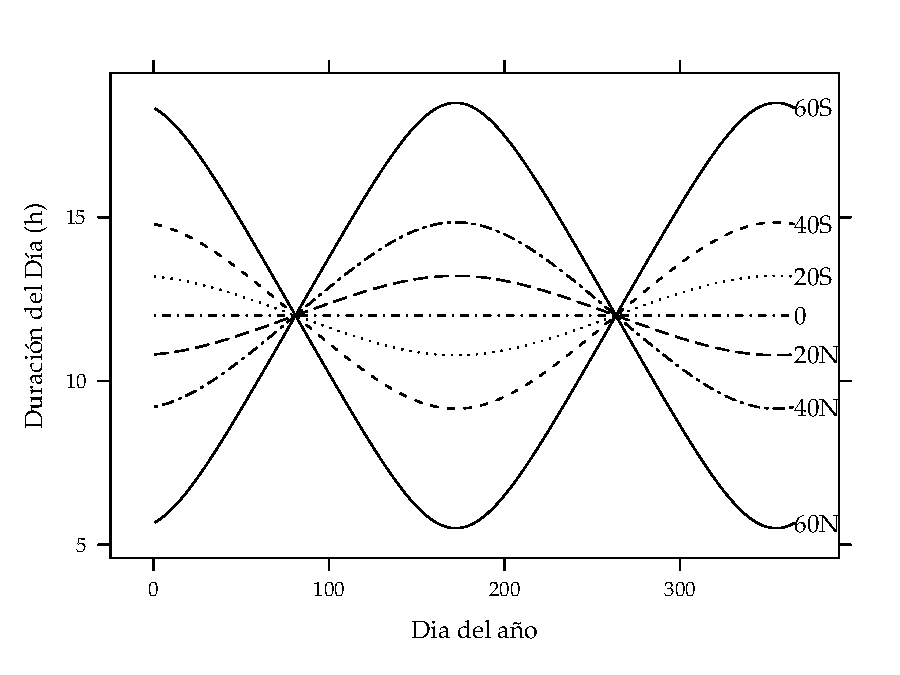
\includegraphics[scale=0.6]{../Figuras/DuracionDia}
    \par\end{center}


\end{frame}

\begin{frame}
  \frametitle{Hora oficial}

  \begin{itemize}
  \item \textbf{La hora oficial} es una medida del tiempo
    \textbf{ligada a un meridiano} que sirve de referencia para una
    zona determinada.
  \item La hora oficial de la España peninsular se rija por el huso
    horario de Centroeuropa. Este huso horario está situado en
    $15\degree\mathrm{E}$.
  \end{itemize}
\end{frame}

\begin{frame}
  \frametitle{Hora oficial}
  \begin{itemize}
  \item \textbf{Corrección}: $\Delta\lambda=\lambda_{L}-\lambda_{H}$,
    con $\lambda_{L}$ la longitud local y $\lambda_{H}$ la longitud
    del huso horario.
  \item Longitudes \emph{positivas} al \emph{este} del meridiano de
    Greenwich.  $\Delta\lambda$ es positiva cuando la localidad está
    situada al este de su huso horario.
  \item Diferencia adicional: \emph{horario de verano}.

  \end{itemize}
\end{frame}

\begin{frame}
  \frametitle{Tiempo solar medio}
  \begin{itemize}
  \item \textbf{La duración del día solar real}, definido como el
    tiempo que transcurre entre dos pasos consecutivos del Sol por el
    meridiano local, \textbf{varía a lo largo del año}.
  \item El promedio anual de esta variación es nulo: \emph{día solar
      medio}, cuya duración es constante a lo largo del año e igual al
    valor medio de la duración del día solar real.
  \end{itemize}
\end{frame}

\begin{frame}
  \frametitle{Ecuación del Tiempo}
  $\mathrm{EoT}=229.18\cdot\left(-0.0334\cdot\sin(M)+0.04184\cdot\sin\left(2\cdot
      M+3.5884\right)\right)$

  \begin{centering}
    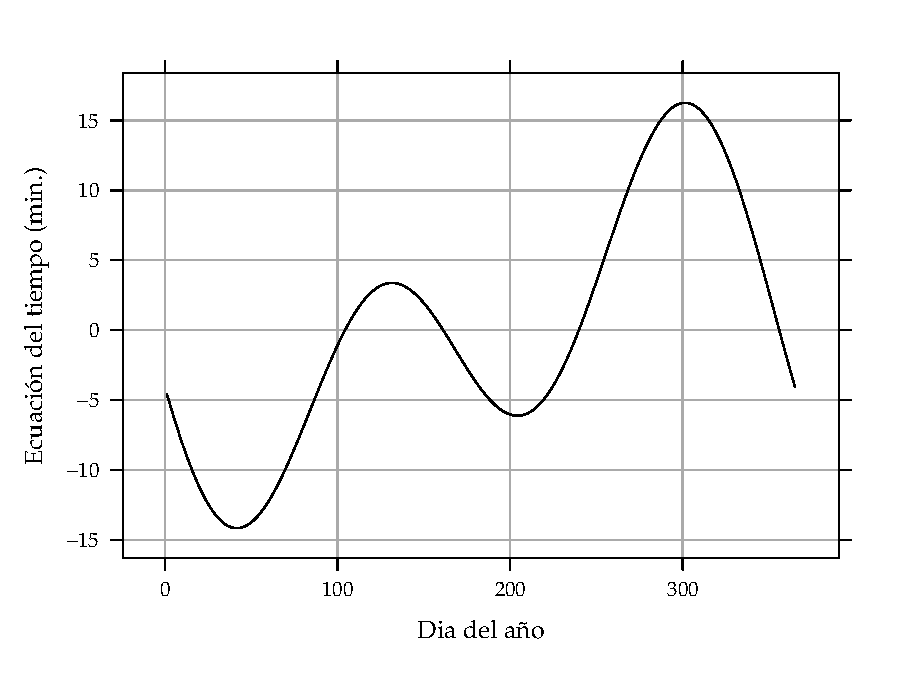
\includegraphics[scale=0.65]{../Figuras/EoT}
    \par\end{centering}

\end{frame}

\begin{frame}
  \frametitle{Ejemplo de cálculo}
  \begin{block}{}
    \[
    \omega=15\cdot(\mathrm{TO}-\mathrm{AO}-12)+\Delta\lambda+\frac{\mathrm{EoT}}{4}\]
  \end{block}
  \begin{itemize}
  \item<1> Calculemos la hora solar real correspondiente al día 23 de
    Abril de 2010 a las 12 de la mañana, hora oficial de la ciudad de
    A Coruña, Galicia.
  \item<2> Esta localidad está contenida en el meridiano de longitud
    $8.38\degree\mathrm{W}$ y su hora oficial está regida por el huso
    horario GMT+1.
  \item<3> Por tanto $\lambda_{L}=-8.38\degree$,
    $\lambda_{H}=15\degree$ y $\Delta\lambda=-23.38\degree$.
  \item<4> En España se aplica el horario de verano y este día está
    incluido en el período afectado, $\mathrm{AO}=1$.
  \item<5> Por último, para este día
    $\mathrm{EoT=\SI{1.78}{\minute}}$.
  \item<6> Así $\omega=-37.94\degree$ (aproximadamente las 9 y media
    de la mañana). El Sol culminará ($\omega=0$) cuando sean las
    14:31, hora oficial.
  \end{itemize}
 
\end{frame}

\begin{frame}
  \frametitle{Cálculo Ángulos Solares}
  \begin{itemize}
  \item Azimut, Ángulo Cenital y Altura Solar, Duración del Dia para
    el:

    \begin{itemize}
    \item Día del Año: 120, 2 horas después del mediodía, Latitud:
      37.2\degree N
    \item Día del Año: 340, 2 horas después del amanecer, Latitud:
      15\degree S
    \end{itemize}
  \item Duración del día 261 del año en las latitudes 10\degree N,
    40\degree N, 70\degree N, 10\degree S, 40\degree S, 70\degree S.
  \item Altura solar en el mediodía del día 25 del año en las
    latitudes 10\degree N, 40\degree N, 10\degree S, 40\degree S.
  \end{itemize}
\end{frame}


\section{Geometría de los sistemas fotovoltaicos}


\begin{frame}[plain]
  \frametitle{Ángulo de Incidencia\\
    Sistema Estático}
\[
\vec{\mu}_{\beta}=[\sin(\beta)\cos(\alpha)]\cdot\vec{\mu}_{h}+[\sin(\beta)\sin(\alpha)]\cdot\vec{\mu}_{\bot}+\cos(\beta)\cdot\vec{\mu}_{c}\]

  \begin{columns}%{}

    \column{4cm}

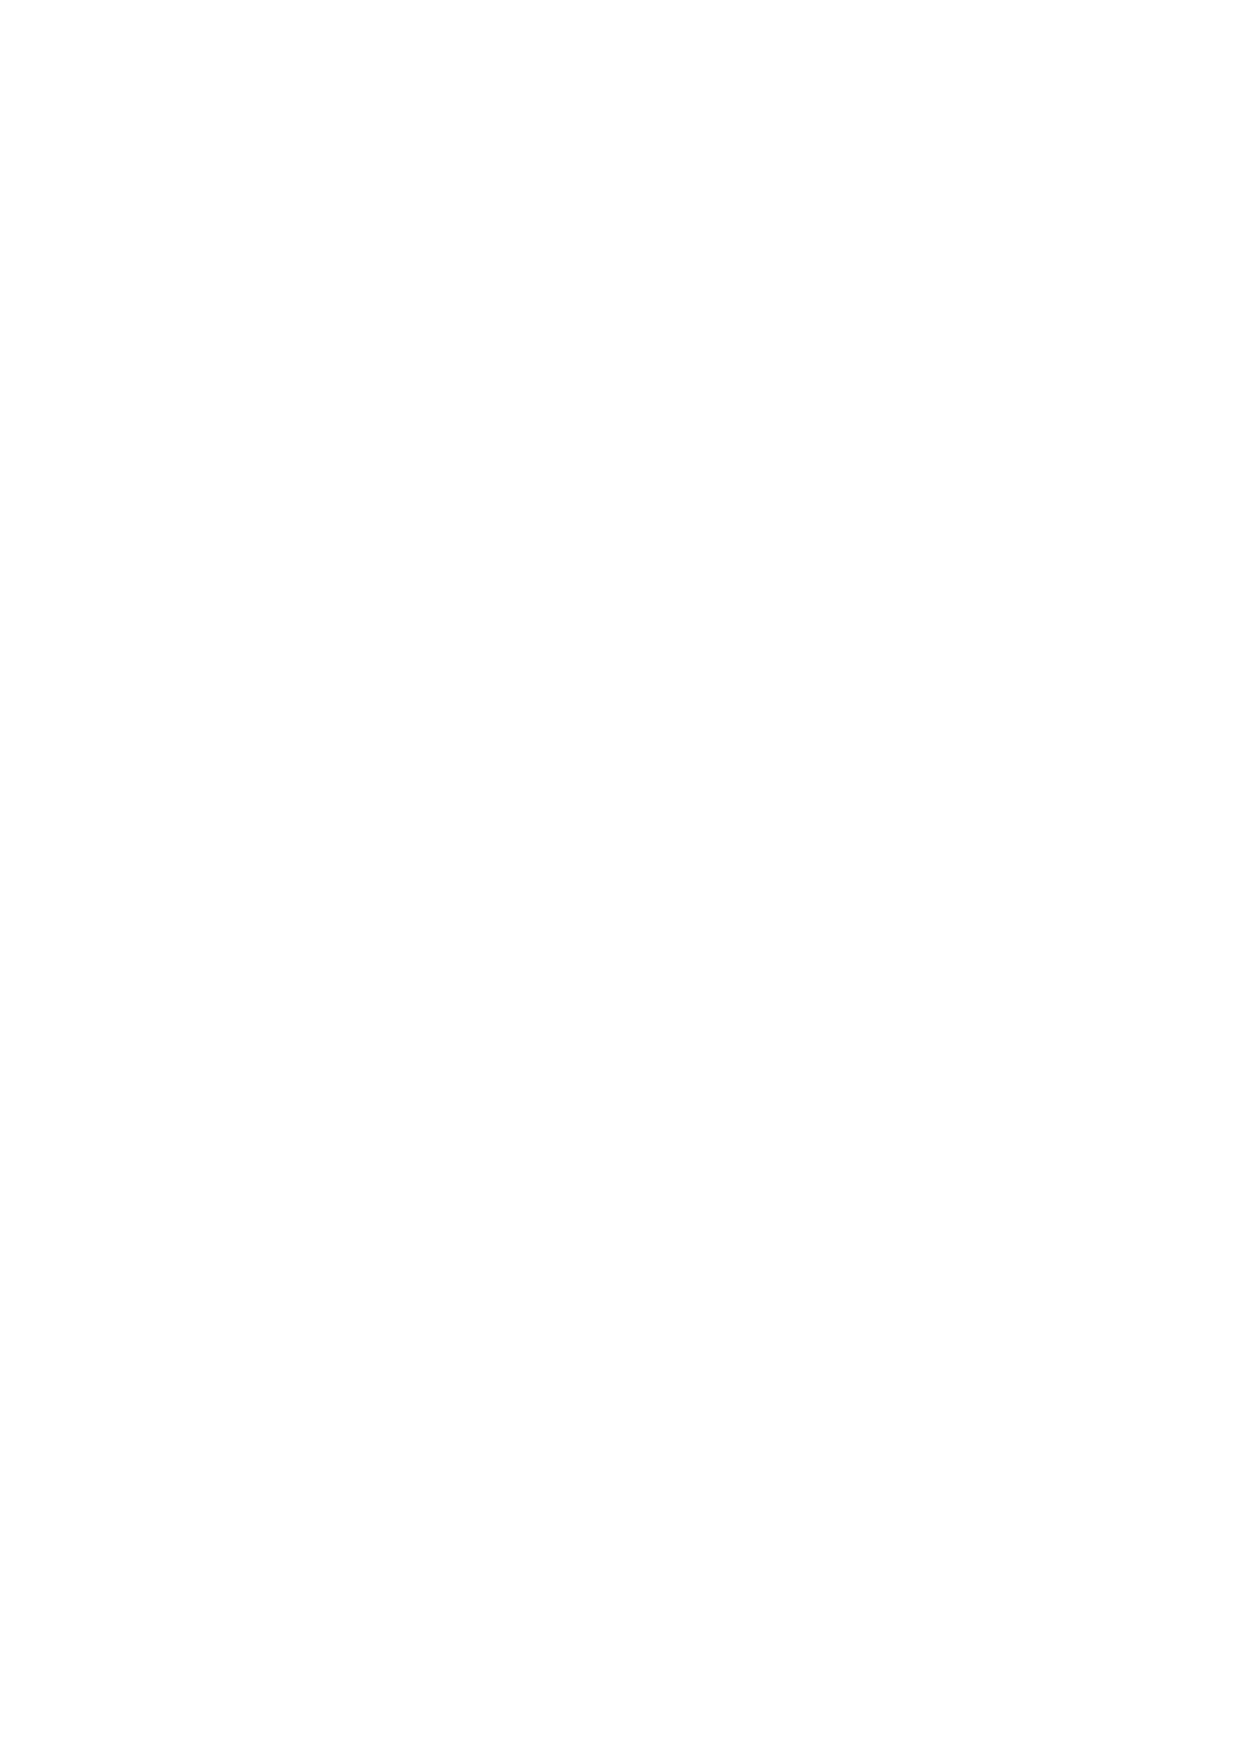
\includegraphics[scale=0.6]{../Figuras/AngulosSistemaEstatico.pdf}


\column{4cm}

{\small 
\begin{align*}
\cos(\theta_{s}) & =\mathrm{signo}(\phi)\cdot\bigl[\sin(\beta)\cos(\alpha)\cos\left(\delta\right)\cos\left(\omega\right)\sin\left(\phi\right)-\nonumber \\
 & -\sin(\beta)\cos(\alpha)\cos\left(\phi\right)\sin\left(\delta\right)\bigr]+\nonumber \\
 & +\sin(\beta)\sin(\alpha)\cos\left(\delta\right)\sin\left(\omega\right)+\nonumber \\
 & +\cos(\beta)\cos\left(\delta\right)\cos\left(\omega\right)\cos\left(\phi\right)+\nonumber \\
 & +\cos(\beta)\sin\left(\delta\right)\sin\left(\phi\right)\label{eq:cosThetaEstatica}\end{align*}
}{\small \par}

\end{columns}%{}

\end{frame}

\begin{frame}[plain]
  \frametitle{Ángulo de Incidencia\\
    Sistema Estático}
  \begin{columns}%{}


    \column{4cm}

    Cuando $\alpha=0$

    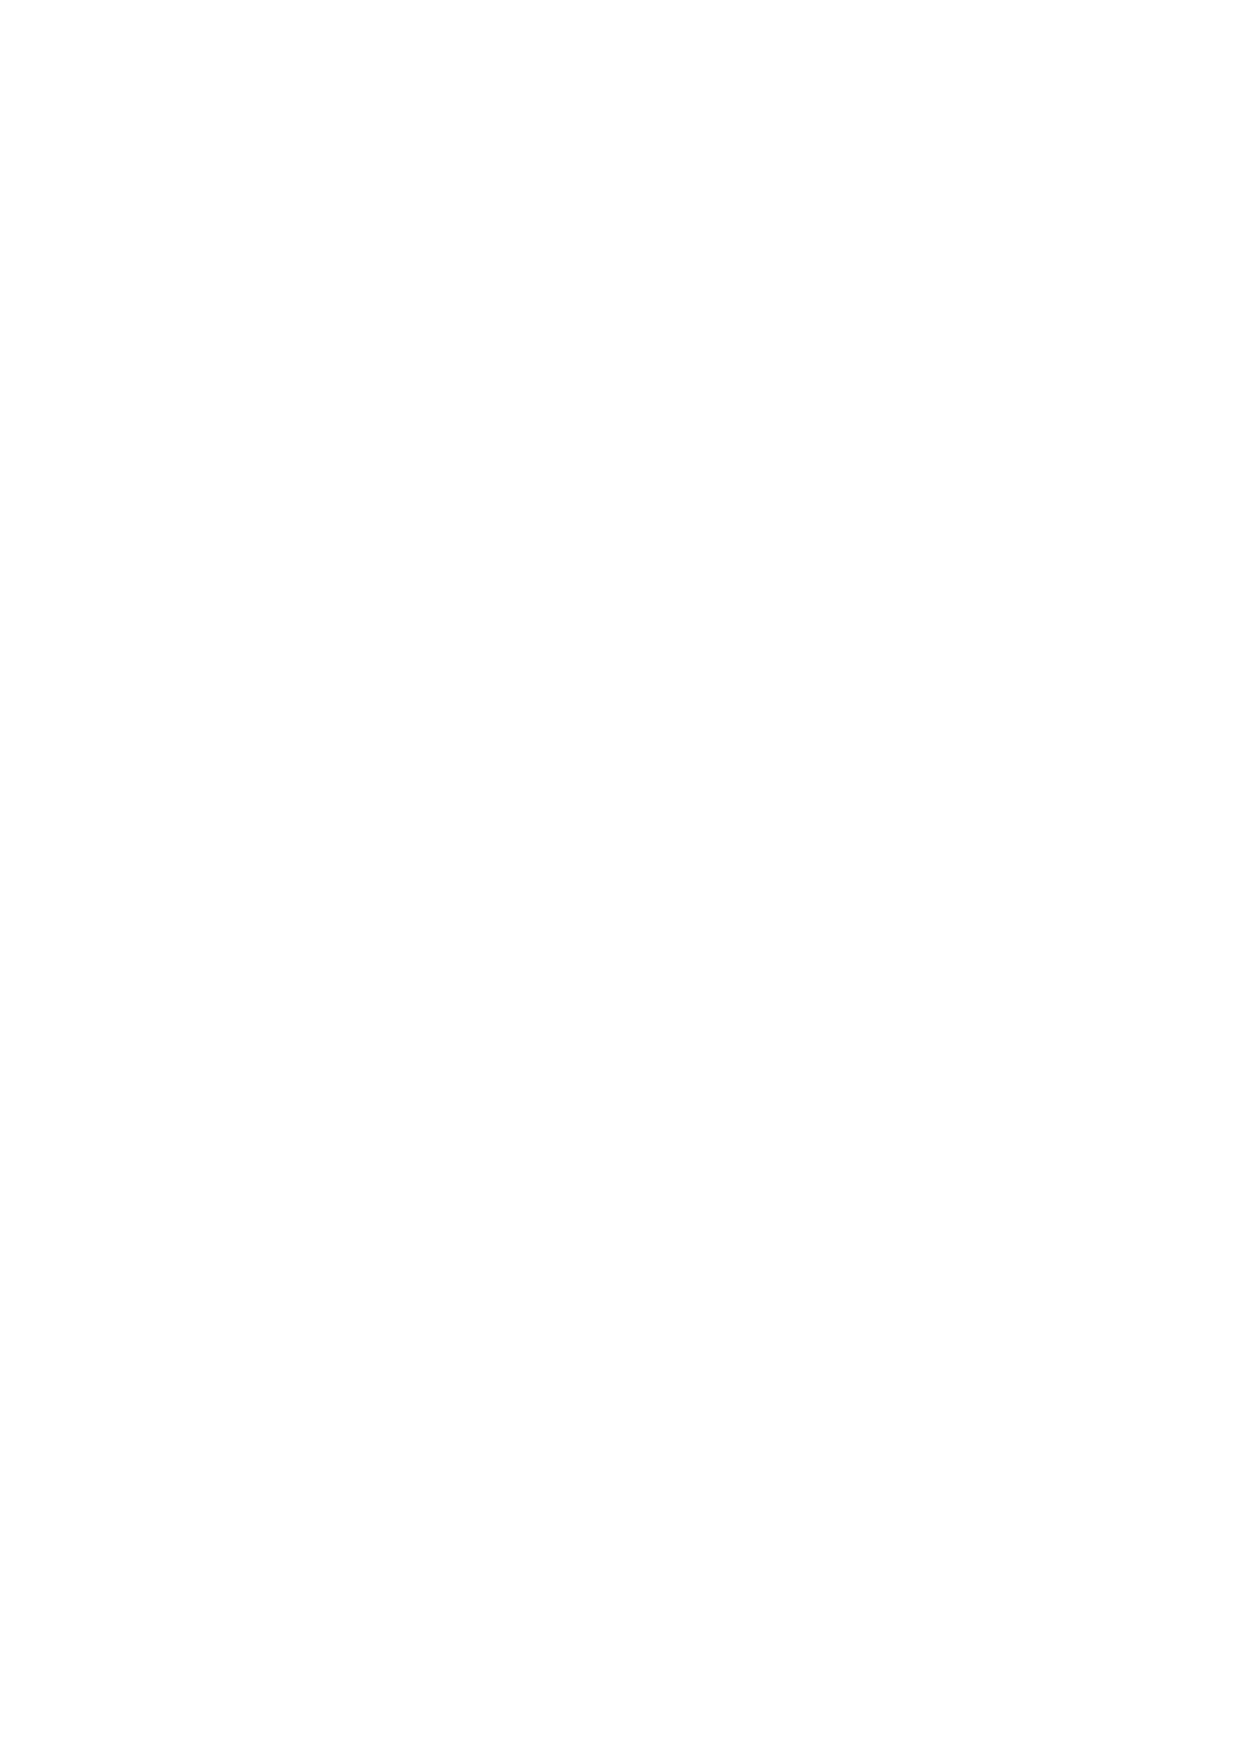
\includegraphics[scale=0.5]{../Figuras/AngulosSistemaEstatico.pdf}


    \column{6cm}
    \begin{align*}
\cos(\theta_{s})& = \cos\left(\delta\right)\cos\left(\omega\right)\cos\left(\beta-|\phi|\right)-\\ 
& - \mathrm{signo}(\phi)\cdot\sin(\delta)\sin\left(\beta-|\phi|\right)
          \end{align*}
  

\end{columns}%{}

\end{frame}


\begin{frame}[plain]
  \frametitle{Ángulo de Incidencia}


  \framesubtitle{Sistema Estático ($40\degree N$)}

  \begin{center}
    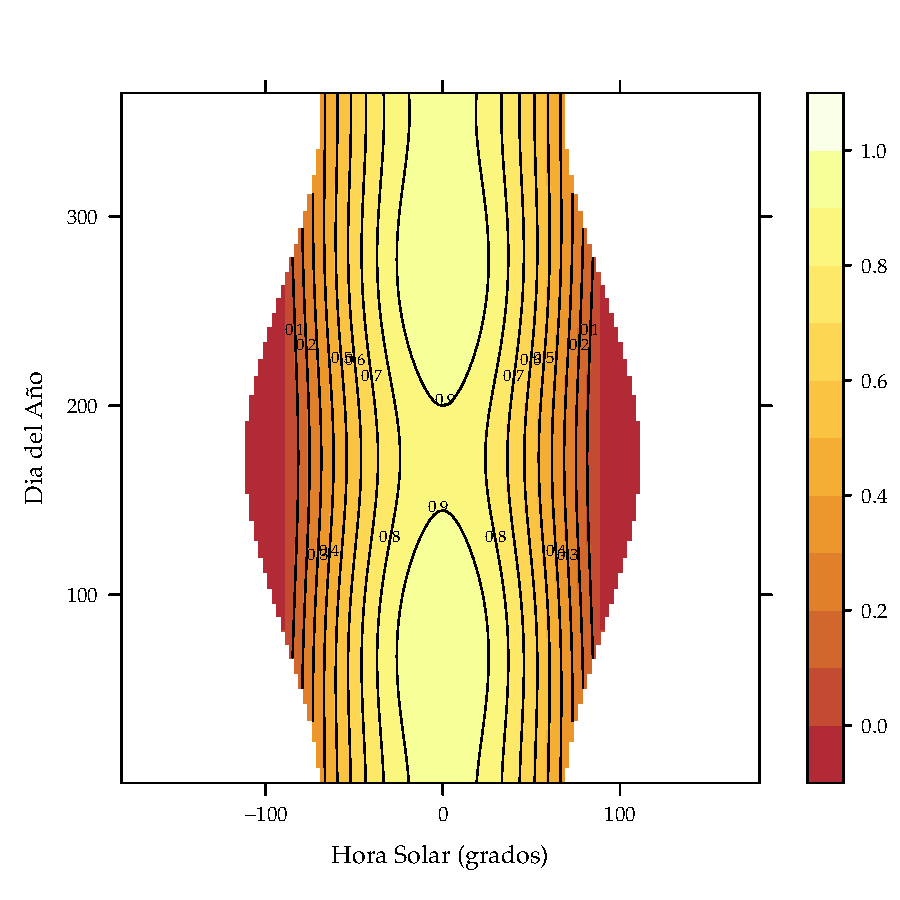
\includegraphics[scale=0.5]{../Figuras/cosThetaEst_40N}
    \par\end{center}


\end{frame}

\begin{frame}[plain]
  \frametitle{Ángulo de Incidencia}


  \framesubtitle{Eje Horizontal N-S, generador horizontal}

\[
\vec{\mu}_{ns}=\sin(\psi_{ns})\cdot\vec{\mu}_{\bot}+\cos(\psi_{ns})\cdot\vec{\mu}_{c}\]


\[
\cos(\theta_{s})=\cos(\delta)\sqrt{\sin^{2}(\omega)+\left(\cos(\omega)\cos(\phi)+\tan(\delta)\sin(\phi)\right)^{2}}\]


\begin{center}
  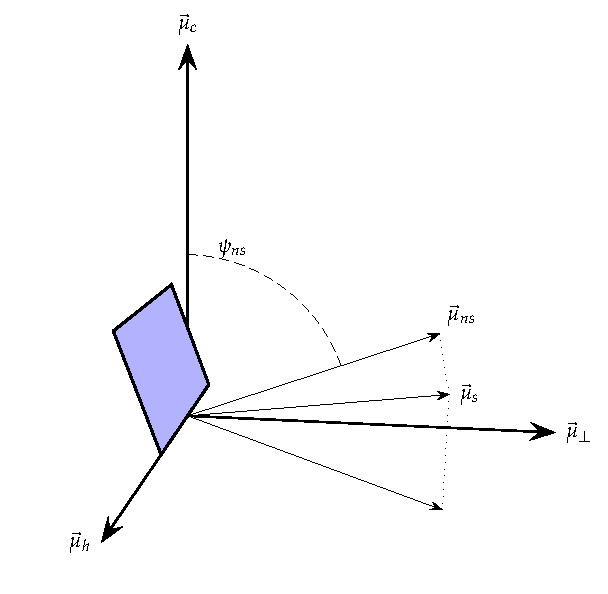
\includegraphics[scale=0.6]{../Figuras/AngulosSistemaHorizontalNS}
  \par\end{center}


\end{frame}

\begin{frame}[plain]
  \frametitle{Ángulo de Inclinación}


  \framesubtitle{Eje Horizontal N-S, generador horizontal, ($40\degree
    N$)}

  \begin{center}
    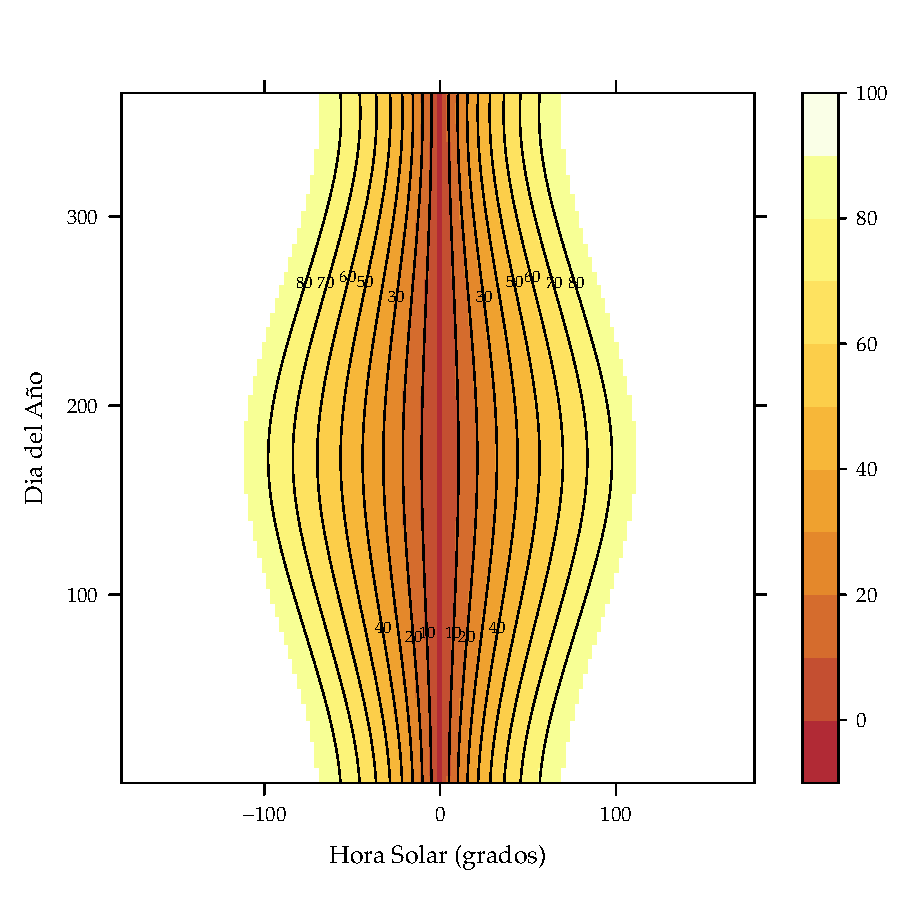
\includegraphics[scale=0.5]{../Figuras/BetaHoriz_40N.pdf}
    \par\end{center}


\end{frame}

\begin{frame}[plain]
  \frametitle{Ángulo de Incidencia}


  \framesubtitle{Eje Horizontal N-S, generador horizontal, ($40\degree
    N$)}

  \begin{center}
    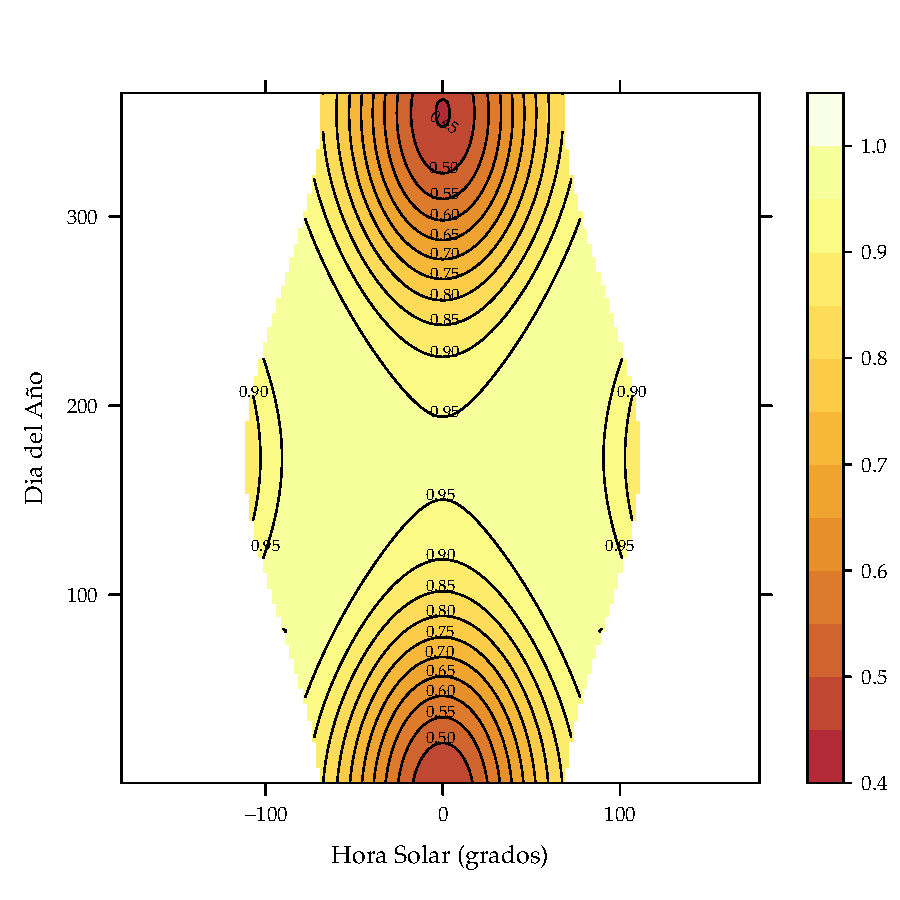
\includegraphics[scale=0.5]{../Figuras/cosThetaHoriz_40N}
    \par\end{center}


\end{frame}

\begin{frame}[plain]
  \frametitle{Ángulo de Incidencia\\
    Acimutal y Doble Eje}
  \begin{columns}%{}


    \column{4cm}
    \begin{block} {Doble Eje}

\begin{align*}
  \beta & =\theta_{z}\\
  \alpha & =\psi_{s}\\
  \cos(\theta_{s}) & =1\end{align*}


\end{block} {}
\begin{block} {Acimutal}

\begin{align*}
  \beta & =cte.\\
  \alpha & =\psi_{s}\\
  \cos(\theta_{s}) & =\cos\left(\beta-\theta_{z}\right)\end{align*}


\end{block}

\column{8cm}

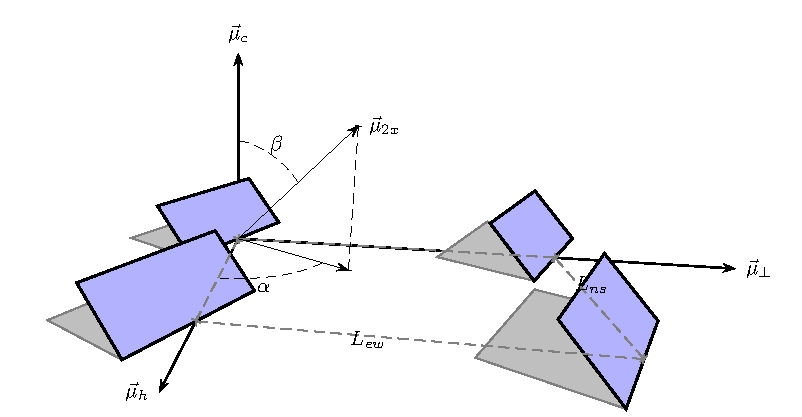
\includegraphics[scale=0.6]{../Figuras/Sombra2X.pdf}

\end{columns}%{}

\end{frame}


\begin{frame}[plain]
  \frametitle{Ángulo de Inclinación}


  \framesubtitle{Doble Eje, ($40\degree N$)}

  \begin{center}
    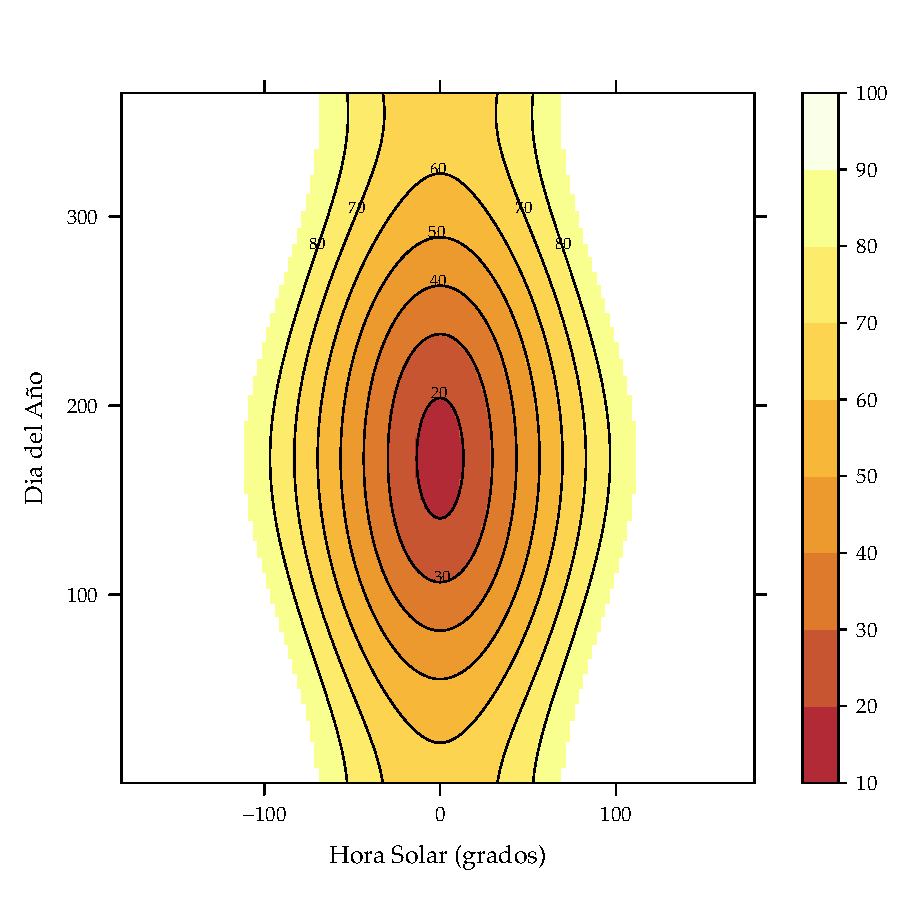
\includegraphics[scale=0.5]{../Figuras/BetaDoble_40N.pdf}
    \par\end{center}


\end{frame}

\begin{frame}[plain]
  \frametitle{Ángulo de Orientación}


  \framesubtitle{Acimutal, ($40\degree N$)}

  \begin{center}
    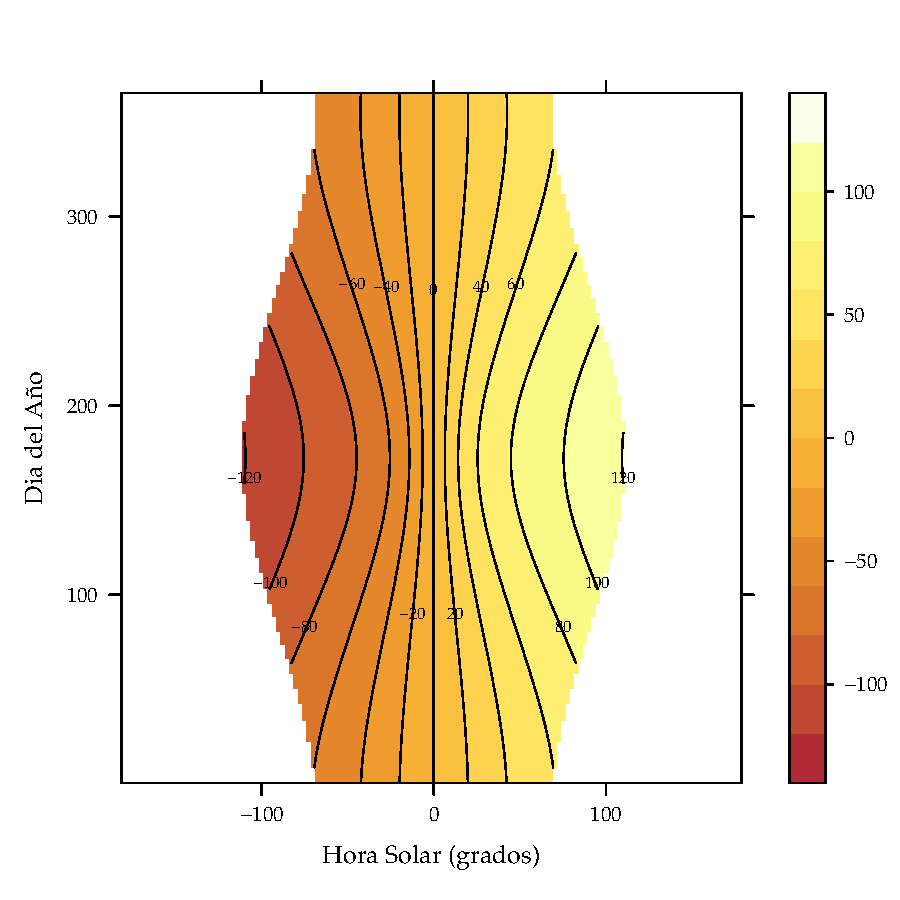
\includegraphics[scale=0.5]{../Figuras/AlfaDoble_40N}
    \par\end{center}


\end{frame}

\begin{frame}[plain]
  \frametitle{Ángulo de Incidencia}


  \framesubtitle{Acimutal, ($40\degree N$)}

  \begin{center}
    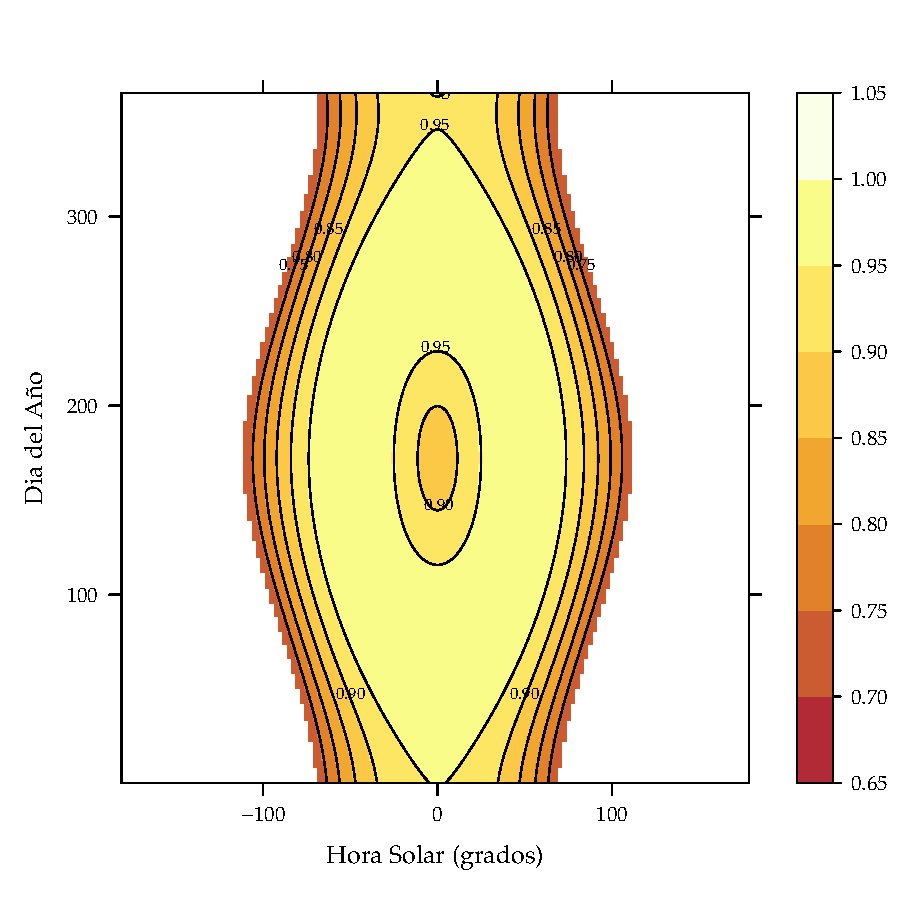
\includegraphics[scale=0.5]{../Figuras/cosThetaAzimutal_40N}
    \par\end{center}


\end{frame}

\begin{frame}
  \frametitle{Cálculo de ángulo de incidencia}
  \begin{description}
  \item [{Para:}]~


    Un sistema estático orientado al Sur y con inclinación de
    30\degree {};

    Un sistema de seguimiento horizontal N-S;

    Un sistema de seguimiento acimutal con inclinación a 35\degree {};

    Un sistema de seguimiento a doble eje,

  \item [{Calcular}] el ángulo de incidencia para el:


    Día del Año: 120, 2 horas después del mediodía, Latitud:
    37.2\degree {}N;

    Día del Año: 340, 2 horas después del amanecer, Latitud: 15\degree
    {}S;

  \end{description}

\end{frame}

\end{document}
